\section{Reflectancia y transmitancia de una monocapa de nanopartículas de materiales reales: oro y plata}
\label{section:AuAg}

Con la finalidad de presentar la respuesta óptica de una monocapa de NPs esféricas hechas con materiales realista, se emplea en esta sección la función dieléctrica con corrección por tamaño para NPs esféricas de oro [Fig. \ref{sfig:sizeAu}] y de plata [Fig. \ref{sfig:sizeAg}]. La elección de NPs de oro y plata surge a partir de su uso de estos materiales par el biosensado \cite{jain2008noble,estevez2014trends}, así como por su biocompatibilidad \cite{fan2009bio,bosetti2002silver}. Se realizaron cálculos de la reflectancia en configuración ATR para monocapas de NPs esféricas de oro y monocapas de NPs esféricas de plata dado que en este esquema, para NPs con una función dieléctrica descrita por el modelo de Drude [Ec. \eqref{eq:Drude}], se identificó un supuesto modo colectivo el cual, si se presenta también en materiales realistas, podría usarse como biosensor. De forma análoga a la sección \ref{ssection:DrudeATR}, se presentan cálculos de la reflectancia  considerando monocapas conformadas por NPs tanto de oro como de plata, variando los parámetros $\Theta$ (fracción de llenado) y  $a$ (radio de las NPs) para identificar y caracterizar al supuesto modo colectivo, así como para optimizar estos parámetros para el biosensado. Adicionalmente, se calcula la transmitancia de las monocapas de NPs de oro y de plata para corroborar que el supuesto modo colectivo presenta características de un modo guiado, como se observó para una monocapa de NPs con una función dieléctrica tipo Drude.

En la Fig.  \ref{fig:Au-R-Theta} se muestran los cálculos de la reflectancia $R$, empleando el CSM, de una monocapa de NPs esféricas idénticas de oro con un radio de $a = 25$ nm, inmersa en una matriz de agua ($n_m = 1.33$) y soportada por un sustrato con un índice de refracción $n_s = 1.5$, que es iluminada por una onda plana en una configuración ATR. La reflectancia se grafica como función del ángulo de incidencia $\theta_i$ y tanto de la longitud de onda $\lambda$ (escala inferior), como de la energía en unidades de $\hbar\omega$ (escala superior). Se consideraron las fracciones de cubierta $\Theta = 0.1,\,0.125,\,0.15,\, 0.175$ y $0.2$ ---garantizando las condiciones de validez del CSM---, así como la polarización de la onda plana incidente: las gráficas \textbf{i)}--\textbf{v)} corresponden a la polarización \emph{p} y \textbf{vi)}--\textbf{x)} a \emph{s}. Las líneas punteadas verticales verdes y rosas corresponden a las SP-SPRs dipolares y cuadrupolares, respectivamente: para una NP de oro de $a= 25$ nm inmersa en agua, la SP-SPR dipolar se localiza en $\lambda \approx 531$ nm y la cuadrupolar en $513$ nm, como se observa en la Fig. \ref{fig:Au-R-Theta}. Los puntos amarillos, localizados a longitudes de onda mayores a las de la SP-SPR dipolar, corresponden al supuesto modo colectivo. A diferencia de los cálculos de la reflectacia de una monocapa de NPs  con una función dieléctrica tipo Drude analizada en la sección \ref{ssection:DrudeATR}, para una monocapa de NPs de oro se observa, adicional a las SP-SPR y al supuesto modo colectivo, excitaciones a valores de $\lambda$ menores a las de las SP-SPRs (líneas verticales punteadas), las cuales corresponden a contribuciones no plasmónicas de la función dieléctrica del oro. Sin embargo, dado que el supuesto modo colectivo se excita a energías menores a las  SP-SPRs, la contribución de los electrones ligados no se traslapa con el supuesto modo colectivo. 

	\begin{figure}[t!]\centering
\hspace*{-.5em}\begin{tikzpicture}[scale=1]
\node[inner sep=0pt] (graf) at (-.15,0){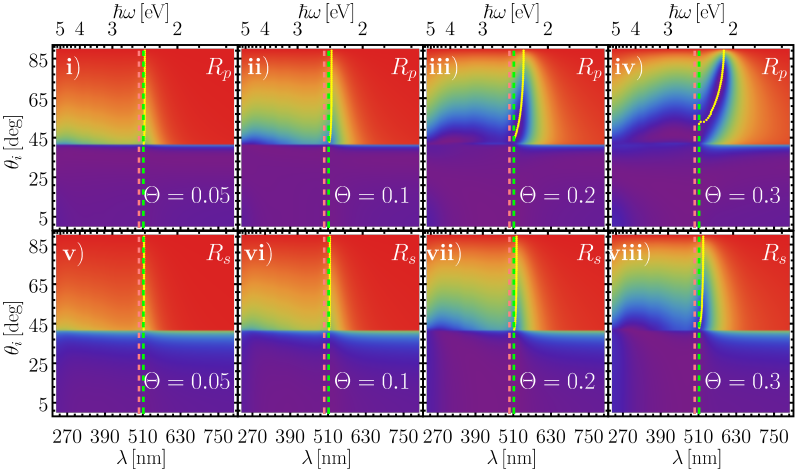
\includegraphics[scale=1]{2-Resultados/figs/6-AuThetaVar/0-2D_Grid}};
\node[right, inner sep=0pt] (legend) at (7.1,.15) {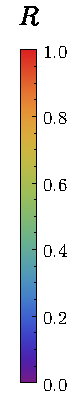
\includegraphics[scale=1, trim={00 -15 00 00}, clip]{2-Resultados/figs/0-RBar_v}};

\def\y{4.2}
	\node at(-5.2,\y){\normalsize $\Theta = 0.10 $};
	\node at(-2.4,\y){\normalsize $\Theta = 0.125 $};
	\node at(0.4,\y) {\normalsize $\Theta = 0.15$};
	\node at(3.2,\y) {\normalsize $\Theta = 0.175 $};
	\node at(6.0,\y) {\normalsize $\Theta = 0.2 $};

\def\xR{6.8}
\def\yR{2.4}	
	\node at(\xR,\yR){$R_p $};
	\node at(\xR,\yR-2.8){$R_s$};
\end{tikzpicture}\vspace*{-.5em}	
	\caption{Gráficas de reflectancia en configuración ATR  de una monocapa de NPs esféricas de oro de radio $a=25$ nm como función del ángulo de incidencia $\theta_i$ y de la longitud de onda $\lambda$ (escala inferior), así como de la energía de la onda plana incidente en unidades de $\hbar\omega$ (escala superior).  Las gráficas   en el renglón superior [$\mathbf{i)-v)}$] muestran los resultados para  polarización \emph{p} y las del renglón inferior  [$\mathbf{vi)-x)}$]  para polarización  \emph{s}, donde se consideraron los valores de fracción de cubierta $\Theta =  0.1,\,0.125,\,0.15,\, 0.175$ y $0.2$.  Las líneas verticales punteadas verdes y rosas corresponden a las SP-SPRs dipolar en $\lambda=531$ nm y  cuadrupolar en $\lambda=513$, respectivamente.  Los puntos amarillos corresponden a los mínimos en $R$ para ángulos mayores a $\theta_c\approx 62.5^\circ$ y longitudes de onda mayores a la SP-SPRs dipolar.
}	\label{fig:Au-R-Theta}	
	\end{figure}	

En la Fig.  \ref{fig:Au-R-Theta}, en las gráficas \textbf{i)}, \textbf{ii)}, \textbf{vi)} y \textbf{vii)}, correspondientes a $\Theta=0.1$ y $0.125$ para ambas polarizaciones, el supuesto modo colectivo se excita a valores de $\lambda$ cercanos a la SP-SPR dipolar para ángulos de incidencia alrededor del ángulo crítico $\theta_c$, sin embargo para valores de $\Theta\geq 1.75$, no es apreciable ningún mínimo en la reflectancia para $\theta_i\approx\theta_c$; por ejemplo para $\Theta=0.2$ para polarización \emph{p} a $\lambda = 531$ nm (línea punteada vertical verde) el supuesto modo colectivo (puntos amarillos) se excita a $\theta\approx 75^\circ$, mientras que para \emph{s} a $65^\circ$. El supuesto modo colectivo para una monocapa de NPs de oro, considerando polarización \emph{p}, no se excita a la longitud de onda de la SP-SPR dipolar para $\Theta\geq 0.175$ a $\theta_i\approx\theta_c$ sin embargo, para polarización \emph{s}, los mínimos en la reflectancia son apreciable para estos valores de $\theta_i$ cuando $\Theta\leq 0.175$, gráficas \textbf{vi)} a \textbf{ix)}. Es decir, a diferencia de los resultados obtenidos al emplear el modelo de Drude para la función dieléctrica de las NPs en la monocapa, el supuesto modo colectivo en una monocapa de NPs de oro no puede excitarse a todos loa ángulos de incidencia a menos que $\Theta\leq 0.15$. Al comparar la respuesta EM de la monocapa, considerando valores de $\Theta$ altos, como $\Theta=0.2$, el corrimiento al rojo del supuesto modo colectivo respecto a la SP-SPR dipolar es mayor  para polarización \emph{p}, \textbf{v)}, que para \emph{s)}, \textbf{x)} ---comportamiento observado, también, al considerar una respuesta tipo Drude para las NPs de la monocapa---. El supuesto modo colectivo se excita en un rango de $\theta_i$ más grande para \emph{s} que para \emph{p}, en particular, a ángulos de incidencia cercanos a $\theta_c$, en donde usualmente operan los biosensores comerciales \cite{svedendahl2009refractometric}.

La reflectancia de una monocapa de NPs con las mismas características que las de la Fig. \ref{fig:Au-R-Theta} pero con NP esféricas de plata, de radio $a=35$ nm, se grafica en la Fig. \ref{fig:Ag-R-Theta}. El radio de las NPs de plata se eligió mayor que el de las NPs de oro para sintonizar las SP-SPRs en el espectro visible: la SP-SPR dipolar corresponde a las líneas verticales verdes en $\lambda=430$ nm y la cuadrupolar, a las líneas verticales rosas en $\lambda=375$ nm. Al igual que para la función dieléctrica del oro, la de la plata cuenta con contribuciones no plasmónicas mas éstas no pueden ser excitadas en el espectro visible, por lo que los cálculos de la reflectancia de una monocapa de NPs de plata se asemejan, en comparación a los de una monocapa de NPs de oro, a los resultados obtenidos al considerar el modelo de Drude-Sommerfeld, como se observa al comparar las Figs. \ref{fig:R-ATR4} (modelo de Drude-Sommerfeld con $\hbar\omega_p=4.3$ eV), \ref{fig:Au-R-Theta} (NPs de oro) y \ref{fig:Ag-R-Theta} (NPs de plata).

\begin{figure}[h!]\centering
\hspace*{-.5em}\begin{tikzpicture}[scale=1]
\node[inner sep=0pt] (graf) at (-.15,0){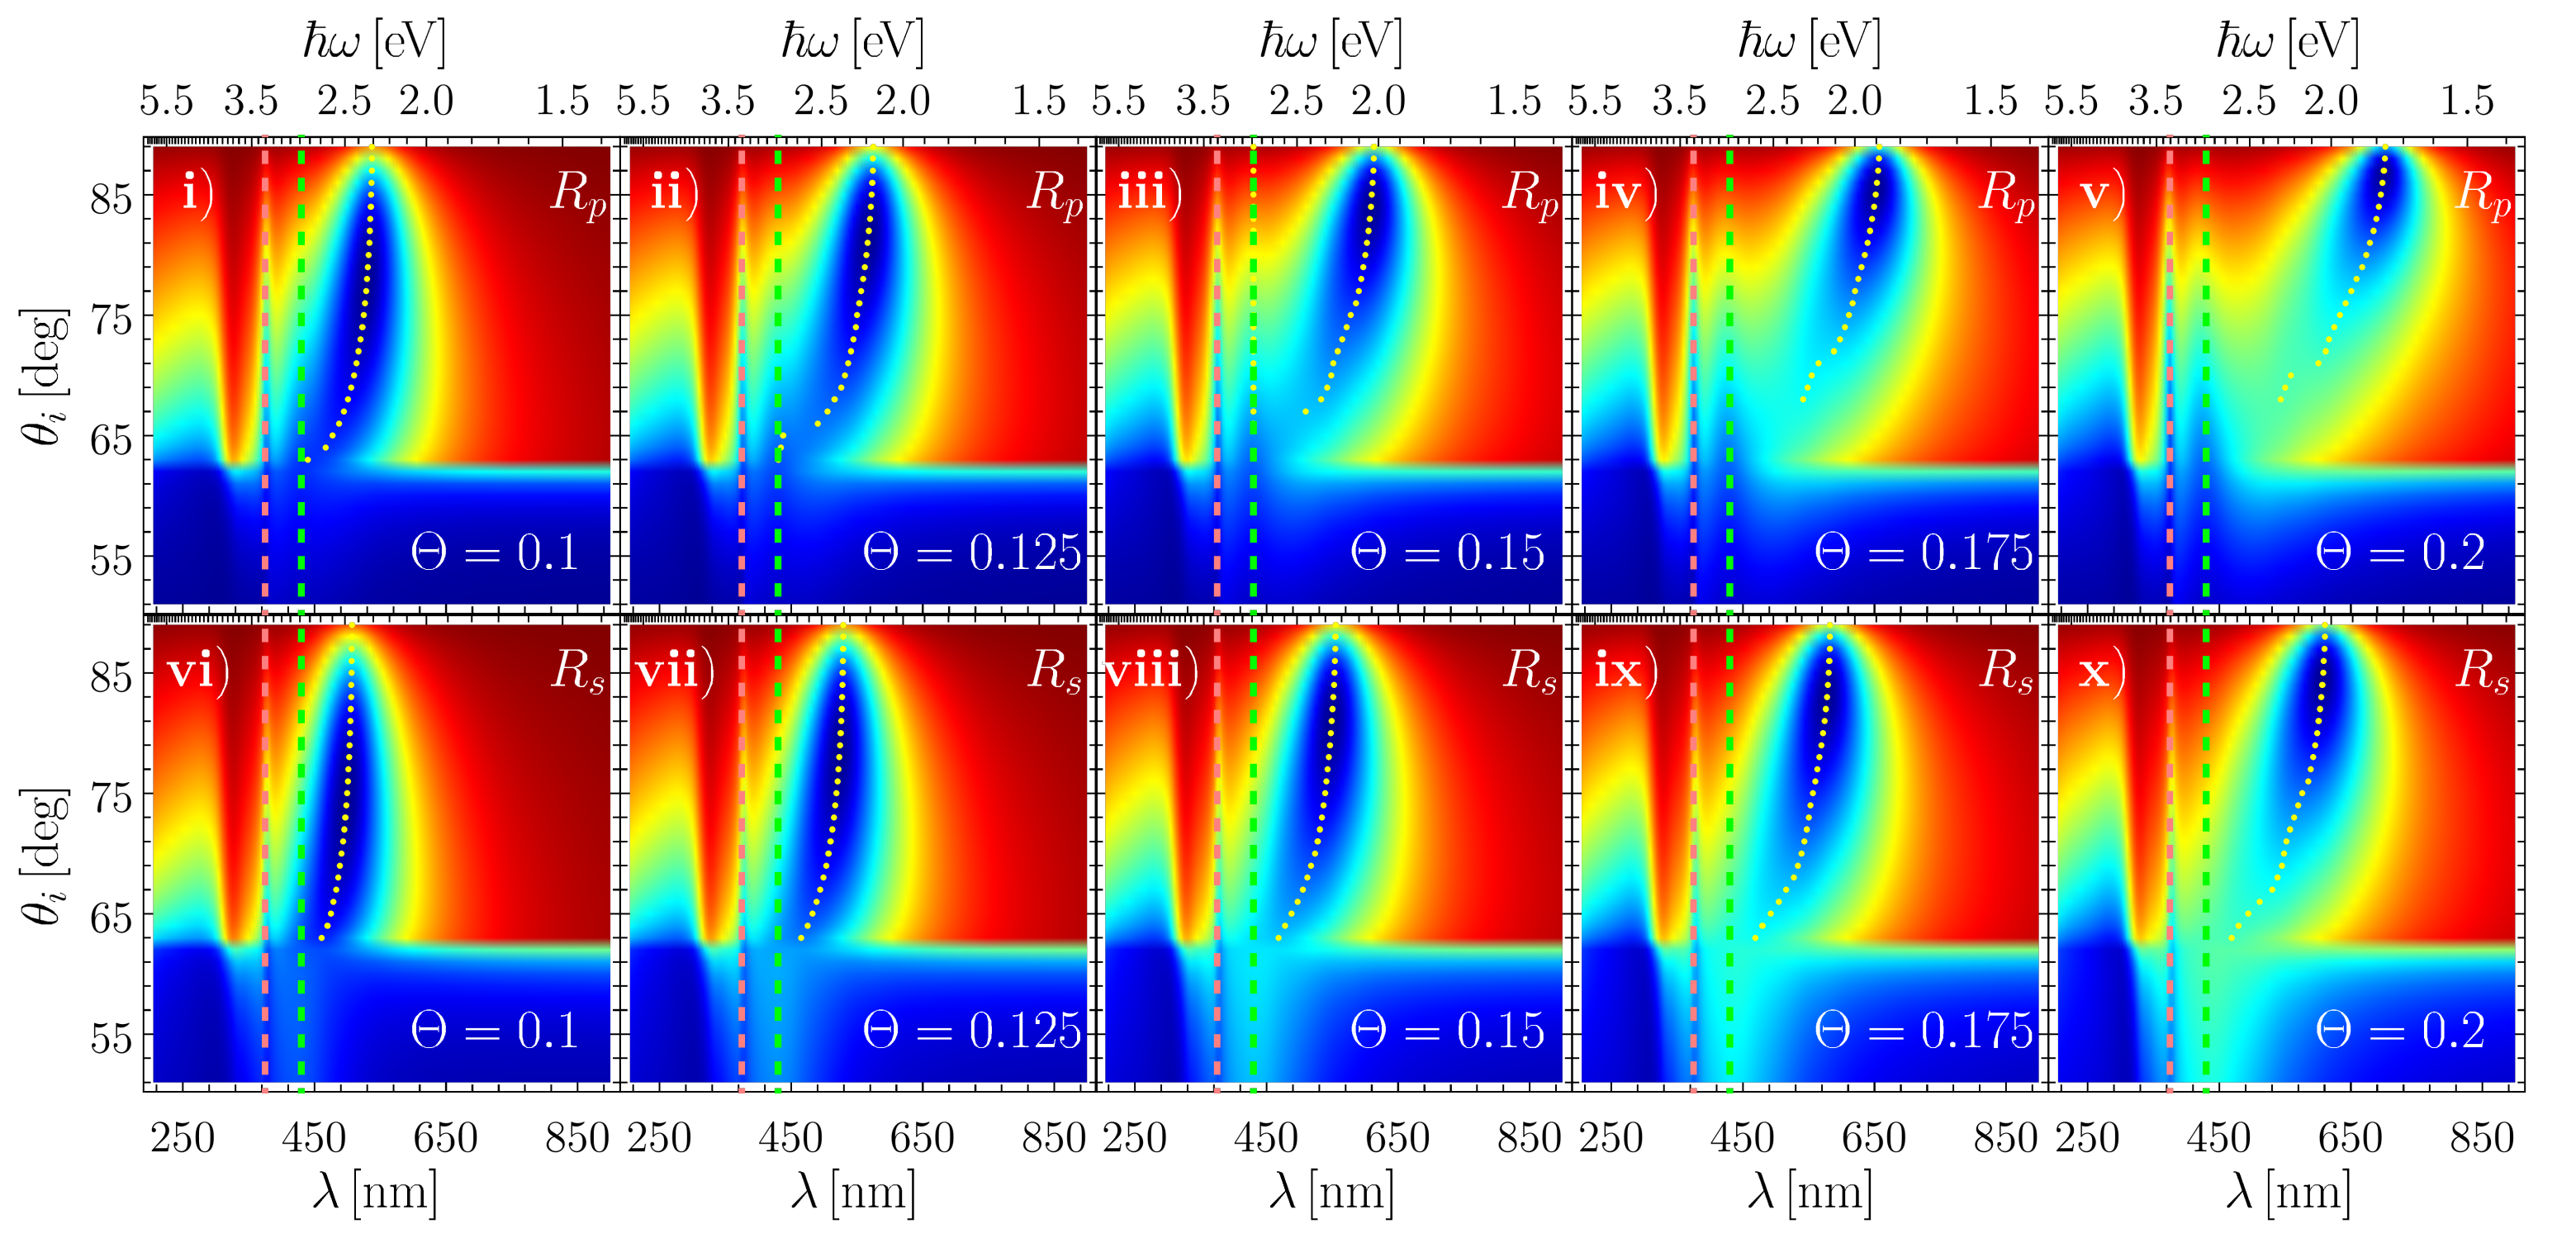
\includegraphics[scale=1]{2-Resultados/figs/7-AgThetaVar/0-2D_Grid}};
\node[right, inner sep=0pt] (legend) at (7.1,.15) {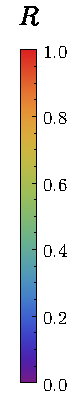
\includegraphics[scale=1, trim={00 -15 00 00}, clip]{2-Resultados/figs/0-RBar_v}};

\def\y{4.2}
	\node at(-5.2,\y){\normalsize $\Theta = 0.10 $};
	\node at(-2.4,\y){\normalsize $\Theta = 0.125 $};
	\node at(0.4,\y) {\normalsize $\Theta = 0.15$};
	\node at(3.2,\y) {\normalsize $\Theta = 0.175 $};
	\node at(6.0,\y) {\normalsize $\Theta = 0.2 $};

\def\xR{7}
\def\yR{2.5}	
	\node at(\xR,\yR){$R_p $};
	\node at(\xR,\yR-2.8){$R_s$};
\end{tikzpicture}\vspace*{-.5em}
	\caption{Gráficas de reflectancia de una monocapa de NPs esféricas de plata de radio $a=35$ nm en configuración ATR como función del ángulo de incidencia $\theta_i$ y de la longitud de onda $\lambda$ (escala inferior), así como de la energía de la onda plana incidente en unidades de $\hbar\omega$ (escala superior).  Las gráficas   en el renglón superior [$\mathbf{i)-v)}$] muestran los resultados para  polarización \emph{p} y las del renglón inferior  [$\mathbf{vi)-x)}$]  para polarización  \emph{s}, donde se consideraron los valores de fracción de cubierta $\Theta = 0.1,\,0.125,\,0.15,\, 0.175$ y $0.2$.  Las líneas verticales punteadas verdes y rosas corresponden a las SP-SPRs dipolar en $\lambda=430$ nm y  cuadrupolar en $\lambda=375$, respectivamente.  Los puntos amarillos corresponden a los mínimos en $R$ para ángulos mayores a $\theta_c\approx 62.5^\circ$ y longitudes de onda mayores a la SP-SPRs dipolar.
}	\label{fig:Ag-R-Theta}	
	\end{figure}	

En la reflectancia para la monocapa de NPs de plata, Fig. \ref{fig:Ag-R-Theta}, la SP-SPR cuadrupolar (línea vertical punteada rosa) se aprecia a $375$ nm para todos los valores de $\Theta$ considerados, sin emabargo, la SP-SPR dipolar (línea punteada vertical verde) sólo se aprecia para polarización \emph{p} cuando $\Theta=0.2$ , gráfica \textbf{v)}, mietras que para \emph{s}, no se aprecia para ningún caso, característica también observada para las NPs con una función dieléctrica tipo Drude en la Fig. \ref{fig:R-RVar}. Otra semejanza entre los resultados obtenidos con el modelo de Drude-Sommerfeld y con las NPs de plata, pero que no se observa con las NPs de oro, es el límite del supuesto modo colectivo cuando $\theta_i$ tiende a $\theta_c$, en donde la longitud de onda de excitación del supuesto modo colectivo tiende a la SP-SPR dipolar.

Tanto para la monocapa de NPs de oro, como de NPs de plata, la reflectancia a las longitudes de onda del supuesto modo colectivo (puntos amarillos en las Figs. \ref{fig:Au-R-Theta} y \ref{fig:Ag-R-Theta}) para  $\Theta\geq 0.15$ es mínima a ángulos de incidencia rasantes ($\theta_i\lessapprox 90^\circ$).  Adicionalmente, el ancho de la resonancia a ángulos rasantes es menor en comparación al resto de los ángulos por lo que podría proponerse localizar al supuesto modo colectivo en $\theta_i>80^\circ$ para ser usado en el biosensado. Sin embargo, en la medición experimental de la reflectancia, el área del haz de luz incidente se deforma (extiende) al incidir sobre la interfaz entre sustrato y la matriz mediate la transformación $A\to A'/\cos\theta_i$, en donde $A$ es el área del haz al incidir sobre la interfaz  y $A'$ es la sección transversal del haz (ver Fig. \ref{fig:hazcircular}). La deformación del haz complica las mediciones a incidencia rasante, restringiendo el valor de $\theta_i$ a ángulos menores a $80^\circ$, valor para el que el diámetro del haz, en la dirección del vector de onda  paralela a la interfaz, aumenta en un factor de $5.7$.

Una diferencia entre los resultados de la reflectancia de las monocapas de NPs de oro y plata, es el valor de $\theta_i$ al cual se comienza a excitar el supuesto modo colectivo una vez escogido $\Theta$, que en el caso  $\Theta=0.15$ es a $\theta_i\approx 65^\circ$ para las NPs de oro y a $\theta_i\gtrapprox\theta_c$ para las de plata. Para analizar este comportamiento, se grafican en la Fig. \ref{fig:AuAg-Cuts-65} cortes de la reflectancia graficada en las Figs. \ref{fig:Au-R-Theta} (para las NPs de oro) y \ref{fig:Ag-R-Theta} (para las NPs de plata) a $\theta_i=65^\circ$. Asimismo, se grafican en la Fig. \ref{fig:AuAg-Cuts-75} cortes de la reflectancia para ambas monocapas a $\theta_i=75^\circ$, ángulo que deforma el área del haz en un factor de $3.8$ y en donde  la reflectancia, evaluada a las longitudes de onda del supuesto modo colectivo para todos los casos de $\Theta$ estudiados en las Figs.  \ref{fig:Au-R-Theta} y  \ref{fig:Ag-R-Theta}, es menor a $0.4$, lo cual permitiría un uso óptimo  del supuesto modo colectivo para el biosensado. En ambas figuras, los paneles izquierdos corresponden a los cálculos para la monocapa de NPs de oro y los derechos a los de plata, mientras que los paneles superiores corresponden a la reflectancia en polarización \emph{p} y los inferiores a polarización \emph{s}. Las líneas punteadas verticales verdes corresponden a la SP-SPR dipola,  que para las NP de oro se localiza en $\lambda\approx 531$ nm y para las de plata en $\lambda\approx 430$ nm; la SP-SPR cuadrupolar (líneas punteadas verticales rosas) se localizan en $\lambda\approx 513$ nm y en $ \lambda\approx 370$ nm para las NPs de oro y plata, respectivamente.

\begin{figure}[h!]\centering
	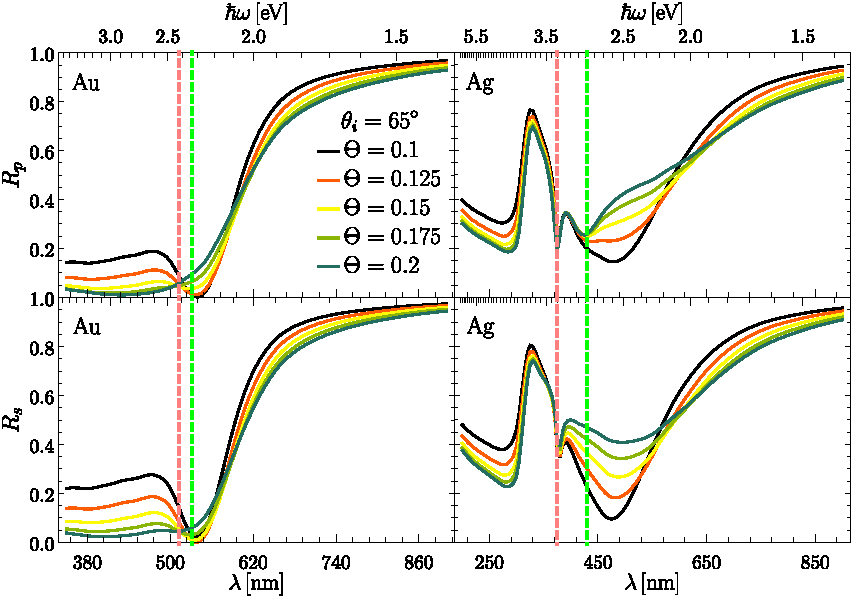
\includegraphics[scale=1]{2-Resultados/figs/6-AuThetaVar/0-cut65_Au_Aug.pdf}\vspace*{-.5em}
	\caption{Cortes a $\theta_i = 65^\circ$ de las gráficas de reflectancia  en configuración ATR  de una monocapa de NPs esféricas de oro de radio $a=25$ nm (Fig. \ref{fig:Au-R-Theta}) y de plata de $a=35$ nm (Fig. \ref{fig:Au-R-Theta}) como función de la longitud de onda $\lambda$ (escala inferior) y de la energía $\hbar\omega$ (escala superior). Los paneles izquierdos corresponden a los cálculos para la monocapa de NPs de oro y los derechos a los de NPs de plata; los panles superiores corresponden a la reflectancia en polarización \emph{p} y los inferiores a polarización \emph{s}. La SP-SPR dipolar (líneas punteadas verticales verdes) para la NP de oro se localiza en  $\lambda \approx 531$ nm y la de la NP de plata en $\lambda\approx430$ nm, mientras la SP-SPR cuadrupolar (líneas punteadas verticales rosas) se localizan en $\lambda\approx513$ nm y en $\lambda\approx370$ nm para las NPs de oro y plara, respectivamente. }\label{fig:AuAg-Cuts-65}
	\end{figure}	
	
%Tanto para la monocapa de NPs de oro como de plata, la reflectancia a valores de $\lambda$ menores a los de la SP-SPR cuadrupolar es menor conforme la fracción de cubierta crece y este comportamiento se invierte para $\lambda$ mayores a la SP-SPR cuadrupolar.
En la Fig. \ref{fig:AuAg-Cuts-65} la reflectancia  para la monocapa de NPs de oro a $\Theta=0.2$  (línea turquesa en los paneles izquierdos) a ambas polarizaciones no se observa la SP-SPR dipolar ($\lambda\approx531$ nm) y tampoco el supuesto modo colectivo. Para $\Theta=0.175$ (línea verde) considerando polarización \emph{p}, ni la SP-SPRs ni el modo colectivo son apreciables pero sí para polarización \emph{s}, en donde excitación del supuesto modo colectivo se superpone a la SP-SPR dipolar, opacándola al ser una excitación más intensa. Para $\Theta= 0.1$ (línea negra)  y $0.125$ (línea naranja), la longitud de onda de excitación del supuesto modo colectivo es $\lambda^{exc} \approx 540\text {nm}$ y la reflectancia evaluada en $\lambda^{exc}$ es $R_p\approx 0$, mientras que  para polarización \emph{s} con $\Theta=0.1$,  $R_s(\lambda^{exc}) \approx0.02$ y, para $\Theta=0.125$, $R_s(\lambda^{exc})\approx 0$; para los valores intermedios de $\Theta$ la reflectancia a las longitudes de onda del supuesto modo colectivo aumenta.

Para la monocapa de NPs de plata, paneles izquierdos en la Fig. \ref{fig:AuAg-Cuts-65}, la reflectancia a $\theta_i=65^\circ$, a todos los valores de $\Theta$, presenta un mínimo a $370$ nm (línea punteada vertical rosa) que corresponde a la SP-SPR cuadrupolar para las NPs de plata empleadas. La excitación dipolar de partícula individual a $430$ nm sólo es apreciable como mínimos en la reflectancia a polarización \emph{p} con $\Theta \geq 0.15$; para valores de fracción de cubierta menores, y para polarización \emph{s}, esta excitación puede observarse, no como un mínimo en $R$, sino como un punto estacionario, es decir, el supuesto modo colectivo y la SP-SPR dipolar se traslapan, cambiando la forma de la resonancia. Los valores de reflectancia para la monocapa de NPs de plata considerando $\theta_i=65^\circ$ son mayores al aumentar $\Theta$ y siempre mayores a $0.2$, a diferencia de los resultados con NPs de oro en donde se obtuvieron valores cercanos a cero. Adicionalmente, el supuesto modo colectivo se corre al rojo al crecer $\Theta$, comportamiento observado en los resultados con NPs con una función dieléctrica tipo Drude pero que no es apreciable para la reflectancia  a  $65^\circ$ de una monocapa de NPs de oro (paneles izquierdos en la Fig. \ref{fig:AuAg-Cuts-65}).
	
	\begin{figure}[h!]\centering
	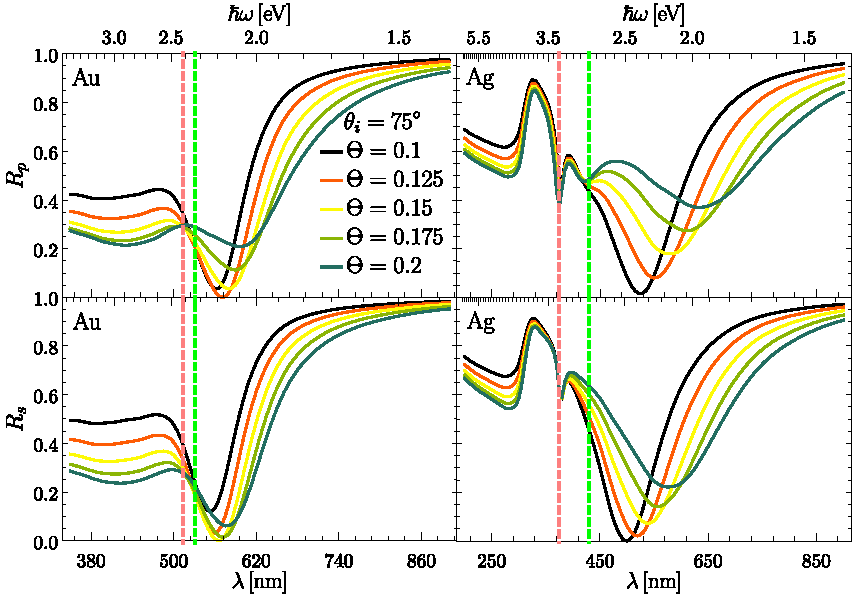
\includegraphics[scale=1]{2-Resultados/figs/6-AuThetaVar/0-cut75_Au_Aug.pdf}\vspace*{-.5em}
	\caption{Cortes a $\theta_i = 75^\circ$ de las gráficas de reflectancia  en configuración ATR  de una monocapa de NPs esféricas de oro de radio $a=25$ nm (Fig. \ref{fig:Au-R-Theta}) y de plata de $a=35$ nm (Fig. \ref{fig:Au-R-Theta}) como función de la longitud de onda $\lambda$ (escala inferior) y de la energía $\hbar\omega$ (escala superior). Los paneles izquierdos corresponden a los cálculos para la monocapa de NPs de oro y los derechos a los de NPs de plata; los panles superiores corresponden a la reflectancia en polarización \emph{p} y los inferiores a polarización \emph{s}. La SP-SPR dipolar (líneas punteadas verticales verdes) para la NP de oro se localiza en  $\lambda \approx 531$ nm y la de la NP de plata en $\lambda\approx430$ nm, mientras la SP-SPR cuadrupolar (líneas punteadas verticales rosas) se localizan en $\lambda\approx513$ nm y en $\lambda\approx370$ nm para las NPs de oro y plara, respectivamente.}\label{fig:AuAg-Cuts-75}
	\end{figure}	

En contraste con los cortes a $\theta_i=65^\circ$ (Fig. \ref{fig:AuAg-Cuts-65}), en la reflectancia para $\theta_i=75^\circ$ (Fig. \ref{fig:AuAg-Cuts-75}) tanto para la monocapa de NPs de oro, como de plata, se aprecia el supuesto modo colectivo a longitudes de onda mayores a la SP-SPR dipolar, además de haberse corrido al rojo respecto al caso de $\theta_i=65^\circ$ para todos los valores de $\Theta$ considerados. Para la monocapa de NPs de oro (paneles izquierdos en la Fig. \ref{fig:AuAg-Cuts-75}), la longitud de onda de excitación del supuesto modo colectivo $\lambda^{exc}$ para $\Theta=0.1$ se localiza en $\lambda\approx570$ nm y en $\lambda\approx550$ nm para polarización \emph{p} y \emph{s}, respectivamente, mientras que para $\theta_i=75^\circ$ se localiza en $\lambda\approx 540$ nm para ambas polarizaciones. Sin embargo, el valor de la reflectancia en $\lambda^{exc}$ aumenta para ambas polarizaciones en comparación con la reflectancia a $\theta_i=65^\circ$. Por otro lado, para la monocapa de NPs de plata, para $\Theta=0.1$ en polarización \emph{p}, el supuesto modo colectivo se corre a $\lambda^{exc}=490$ nm al evaluarse en $\theta_i=75^\circ$, mientras que para $\theta_i=65^\circ$ se localizaba en $470$ nm; para polarización \emph{s}, el supuesto modo colectivo a $75^\circ$ se encuentra a $\lambda^{exc}=470$ y a $65^\circ$ a $455$ nm; adicionalmente $R(\lambda^{exc})\approx 0$ para $\theta_i=75^\circ$, es decir, que es menor en comparación al caso de $\theta_i=65^\circ$. El corrimiento al rojo de $\lambda^{exc}$ es un comportamiento observado para todos los valores de $\Theta$ para ambas monocapas.

Otra característica compartida por todos los casos estudiados de $\Theta$, al comparar los cortes para $\theta_i=65^\circ$ (Fig. \ref{fig:AuAg-Cuts-65}) y para $\theta_i=75^\circ$ (Fig. \ref{fig:AuAg-Cuts-75}), es una mejor definición en la forma de la resonancia y de su FWHM. Por ejemplo, para la monocapa de NPs de plata, para los dos ángulos de incidencia escogidos y el caso de $\Theta=0.2$ (líneas turquesas en los paneles izquierdos inferiores), la resonancia es menos amplia y mejor definida para $\theta_i=75^\circ$ que para $\theta_i=65^\circ$. Lo análogo sucede para la monocapa de NPs de oro al considerar fracciones de cubierta mayores s $0.175$.% En contraste, los valores de la reflectancia a $\lambda^{exc}$ para la monocapa de NPs de oro y de plata no son similares: para las NPs de oro, $R_p\approx 0$ cuando $\Theta=0.125$ (línea naranja) y $R_s\approx 0$ para $\Theta=0.15$ (línea amarilla) mas para las NPs de plata $R\approx 0$, para ambas polarizaciones, cuando $\Theta=0.1$ (línea negra). Es decir, para los valores de fracciones de cubierta $\Theta$ escogidos, considerando NPs de oro de de $25$ nm y de plata de $35$ nm, la optimización de la monocapa para el biosensado es distinta.

Para determinar si los radios elegidos para las NPs de oro y de plata son los óptimos para el empleo del supuesto modo colectivo en el sensado. Se presentan a continuación 	gráficas de la reflectancia en configuración ATR para una monocapa de NPs de oro (Fig. \ref{fig:Au-R-Rad}) y de plata (Fig. \ref{fig:Ag-R-Rad}) para un valor de fracción de cubierta $\Theta $fijo y para disintos radios $a$ de las NPs. En la Fig. \ref{fig:Au-R-Rad} se grafica la reflectancia en configuración ATR para una monocapa de NPs de oro, inmersa en un medio con $n_m=1.33$ y soportada por un sustrato con $n_s=1.5$ considerando  $\Theta=0.125$, elegida con base en los resultados calculados en las Figs. \ref{fig:AuAg-Cuts-65} y \ref{fig:AuAg-Cuts-75}, y donde se varían los radios de las NPs alrededor de $25$ nm, es decir, $a=15$ nm, $20$ nm, $25$ nm, $30$ nm y $35$ nm, siendo entonces las SP-SPR dipolares (líneas punteadas verticales verdes) $525$ nm, $527$ nm, $531$ nm, $535$ nm y $541$ nm para cada radio, respectivamente, y las cuadrupolares (líneas punteadas verticales rosas) $513$ nm para $a=15$ nm, $20$ nm y $25$ nm, y $514$ nm para $a=30$ nm y $35$ nm; el supuesto modo colectivo se representa mediante los punto amarillos.

\begin{figure}[t!]\centering
\hspace*{-.5em}\begin{tikzpicture}[scale=1]
\node[inner sep=0pt] (graf) at (-.15,0){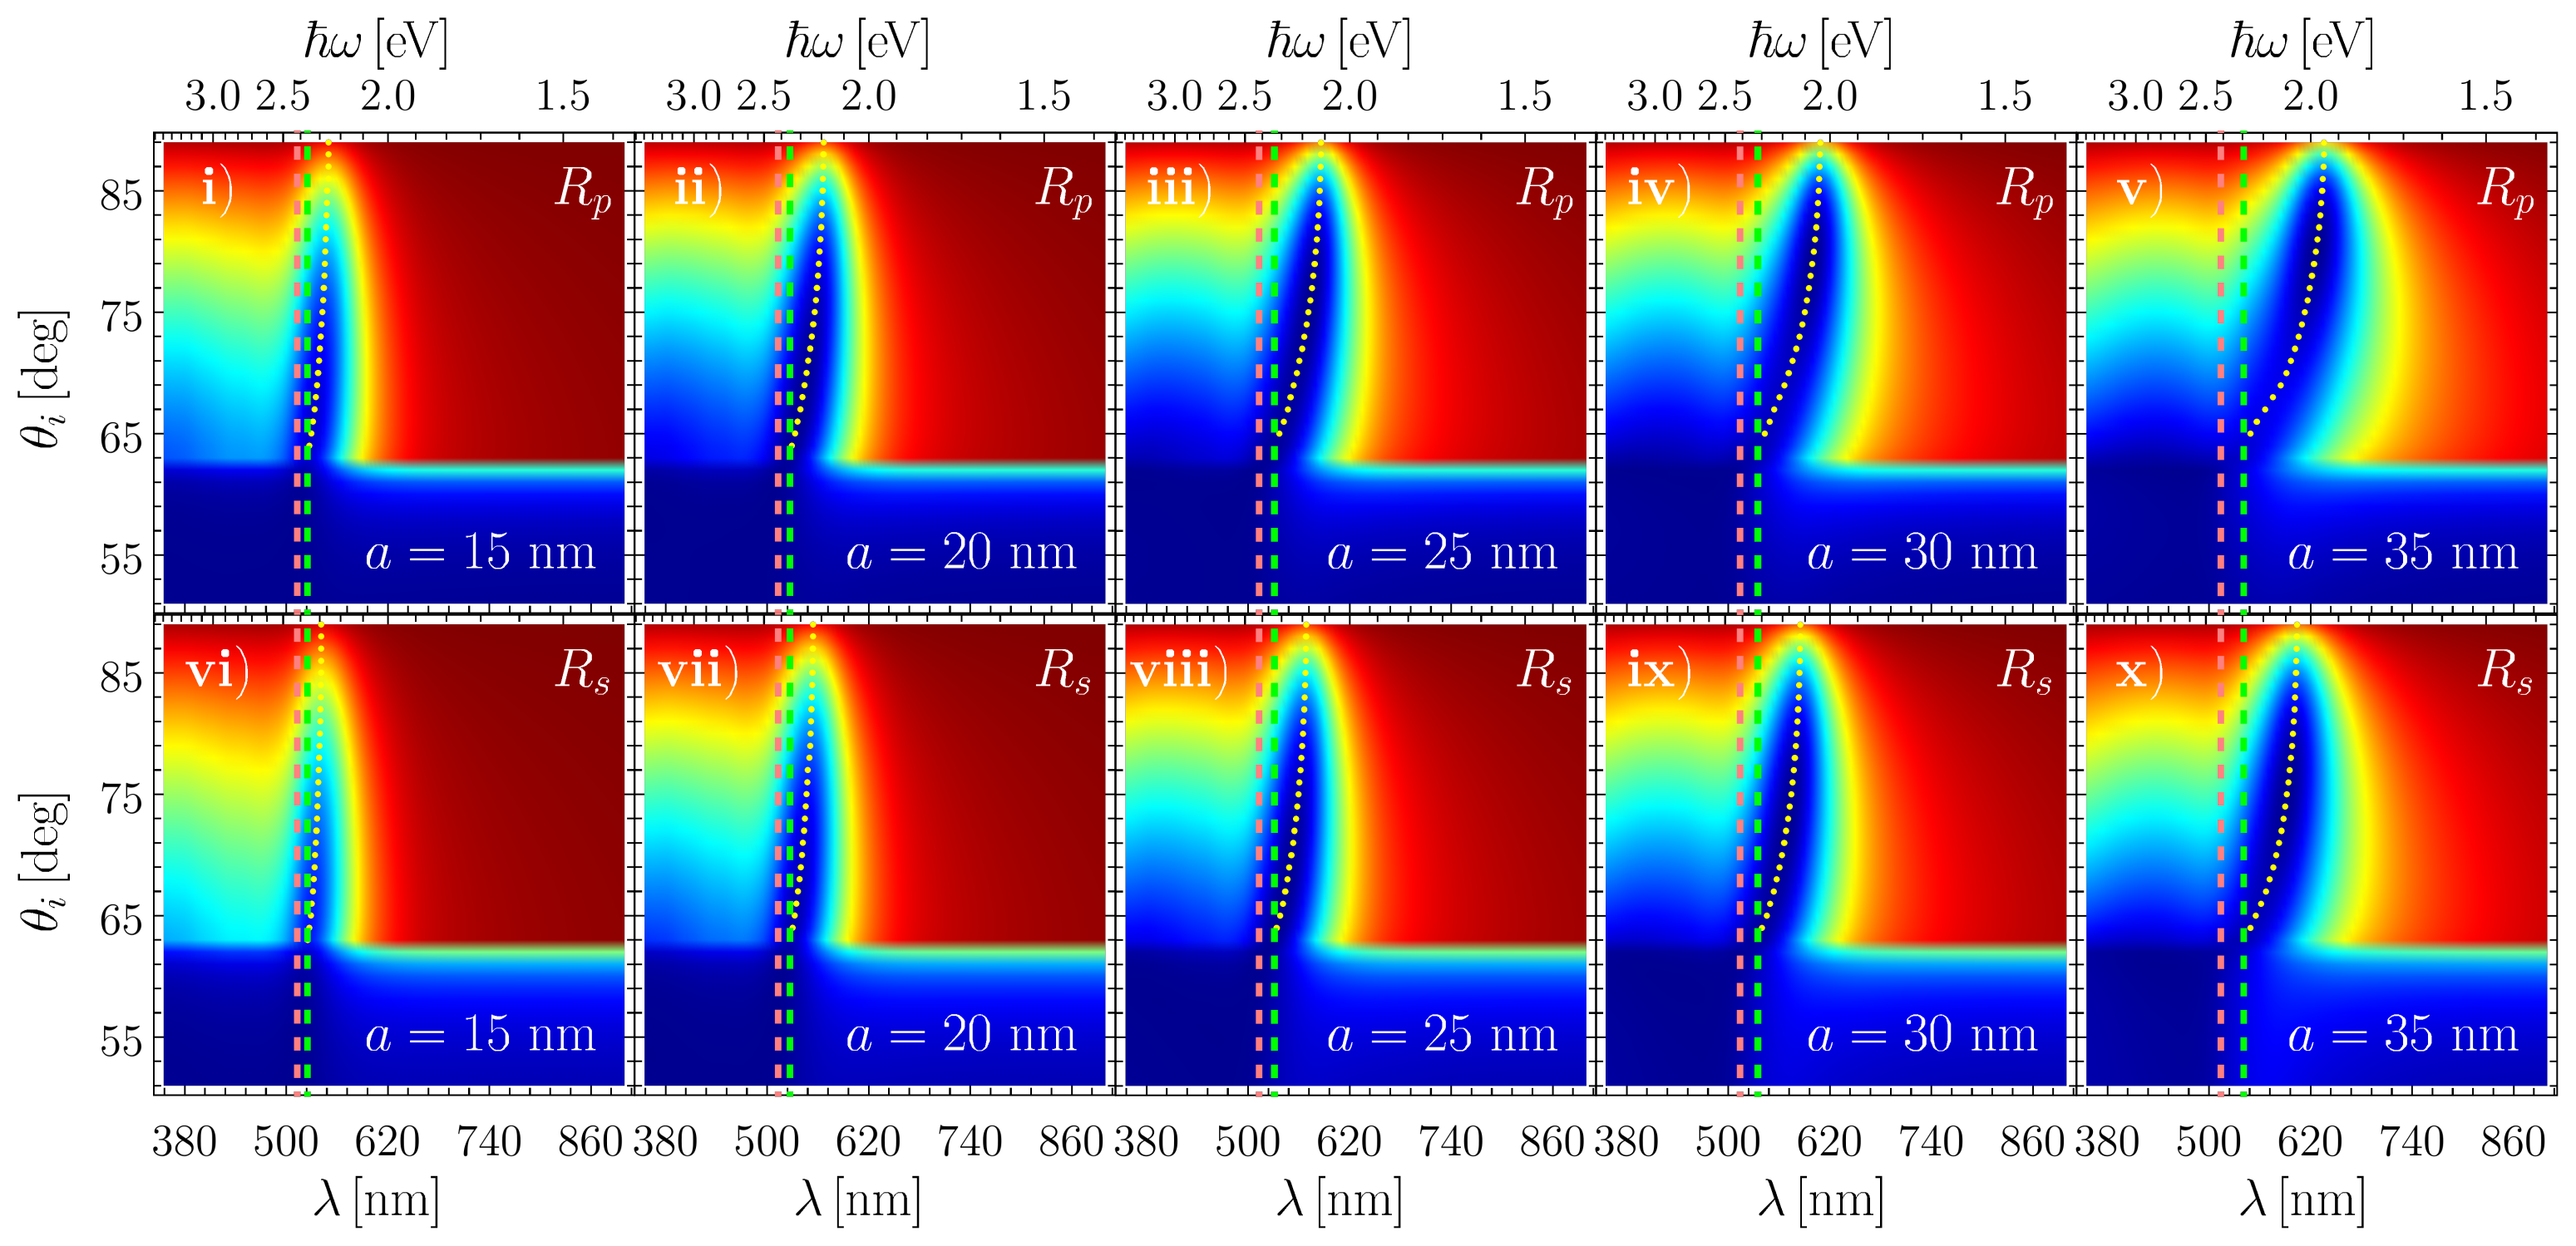
\includegraphics[scale=1]{2-Resultados/figs/8-AurVar/0-2D_Grid}};
\node[right, inner sep=0pt] (legend) at (7.1,.15) {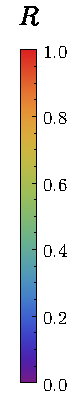
\includegraphics[scale=1, trim={00 -15 00 00}, clip]{2-Resultados/figs/0-RBar_v}};

\def\y{4.2}
	\node at(-5.2,\y){\normalsize $a = 15 $ nm};
	\node at(-2.4,\y){\normalsize $a = 20 $ nm};
	\node at(0.4,\y) {\normalsize $a = 25$ nm};
	\node at(3.2,\y) {\normalsize $a = 30 $ nm};
	\node at(6.0,\y) {\normalsize $a = 35 $ nm};

\def\xR{7}
\def\yR{2.5}	
	\node at(\xR,\yR){$R_p $};
	\node at(\xR,\yR-2.8){$R_s$};
\end{tikzpicture}\vspace*{-.5em}
	\caption{Gráficas de reflectancia de una monocapa de NPs de oro en configuración ATR como función del ángulo de incidencia $\theta_i$ y de la longitud de onda $\lambda$ (escala inferior), así como de la energía  $\hbar\omega$ (escala superior).  Las gráficas   en el renglón superior [$\mathbf{i)-v)}$] muestran los resultados para  polarización \emph{p} y las del renglón inferior  [$\mathbf{vi)-x)}$]  para polarización  \emph{s}, donde se consideró una fracción de cubierta $\Theta = 0.123$ y  NPs de radio  $a$: $20$ nm, $25$ nm, $30$ nm y $35$ nm.  Las líneas verticales punteadas verdes y rosas corresponden a las SP-SPRs dipolar y  cuadrupolar, respectivamente.  Los puntos amarillos corresponden a los mínimos en $R$ para ángulos mayores a $\theta_c\approx 62.5^\circ$ y longitudes de onda mayores a la SP-SPRs dipolar.
}	\label{fig:Au-R-Rad}	
	\end{figure}	


En la Fig. \ref{fig:Au-R-Rad} se observa la tendencia identificada con la monocapa de NPs con una función dieléctrica tipo Drude al variar el tamaño de las NPs: a radios $a$ mayores, el supuesto modo colectivo se corre al rojo y el ancho de la resonancia aumenta; conforme el radio disminuye, el supuesto modo colectivo se empalma con la SP-SPR dipolar. Al comparar la respuesta EM de la monocapa de NPs de oro ante variaciones de fracción de cubierta (Fig. \ref{fig:Au-R-Theta})  el supuesto modo colectivo a la longitud de onda de la SP-SPR dipolar se excita a partir de un ángulo de incidencia, el cual aumenta conforme $\Theta$ crece. Por otro lado, al considerar el parámetro $\Theta$ fijo y variar el radio de las NPs (Fig. \ref{fig:Au-R-Rad}), el supuesto modo colectivo se excita, a la longitud de onda de la SP-RPR dipolar,  a partir del mismo ángulo de incidencia ($\theta_i\approx 65^\circ$) para todos los valores de $a$ considerados.

En la Fig. \ref{fig:Ag-R-Rad}	 se presentan los cálculos de la reflectancia de una monocapa de NPs  de plata, inmersa en un medio con $n_m=1.33$ y soportada por un sustrato con $n_s=1.5$ en configuración ATR. Se considera  $\Theta=0.1$,  según el análisis de las Figs. \ref{fig:AuAg-Cuts-65} y \ref{fig:AuAg-Cuts-75}, y los radios de las NPs alrededor de $35$ nm, es decir, $a=30$ nm, $35$ nm, $40$ nm, $45$ nm y $50$ nm, siendo entonces las SP-SPR dipolares (líneas punteadas verticales verdes) localizadas en $\lambda\approx 417$ nm, $\lambda\approx 430$ nm, $\lambda\approx 444$ nm, $\lambda\approx 459$ nm y $\lambda\approx 479$ nm para cada radio, respectivamente, y las cuadrupolares (líneas punteadas verticales rosas) en $\lambda\approx 373$ nm, $\lambda\approx 376$ nm, $\lambda\approx 379$ nm, $\lambda\approx 383$ nm y $\lambda\approx 388$ nm, respectivamente; los puntos amarillos corresponden al supuesto modo colectivo. El comportamiento del supuesto modo colectivo es semejante al observado para el oro en la Fig. \ref{fig:Au-R-Rad}: al aumentar el radio de las NPs, el supuesto modo colectivo es más apreciable y se corre hacia el rojo, efecto más evidente para polarización \emph{p} que para \emph{s}, mientras que el ensanchamiento del supuesto modo colectivo es mayor para las NPs de plata debido a que el radio de las NPs es mayor que el de las NPs de oro.

Para contrastar con los cortes de la reflectancia a $\theta_i=65^\circ$ y $75^\circ$, cuando se varió el valor de la fracción se cubierta para un radio fijo, se grafican en la Fig. \ref{fig:AuAg-Cuts-Rad-65} cortes a $\theta_i = 65^\circ$  y en la  Fig.  \ref{fig:AuAg-Cuts-Rad-75} a $75^\circ$ de la reflectancia $R$ de las Figs. \ref{fig:Au-R-Rad} y \ref{fig:Ag-R-Rad}, con la finalidad de observar a qué longitud de onda se sintoniza el supuesto modo colectivo a los valores de $\theta_i$ seleccionados, así como el ancho de su resonancia, y escoger los parámetros óptimos para su uso en el sensado. Tanto en la Fig. \ref{fig:AuAg-Cuts-Rad-65}, como en la Fig. \ref{fig:AuAg-Cuts-Rad-75}, los paneles izquierdos corresponden a los cálculos para una monocapa de NPs de oro con $\Theta=0.125$ y los derechos para una monocapa de NPs de plata con $\Theta=0.1$, y los paneles superiores a polarización \emph{p} y los inferiores a \emph{s}.

\begin{figure}[h!]\centering
\hspace*{-.5em}\begin{tikzpicture}[scale=1]
\node[inner sep=0pt] (graf) at (-.15,0){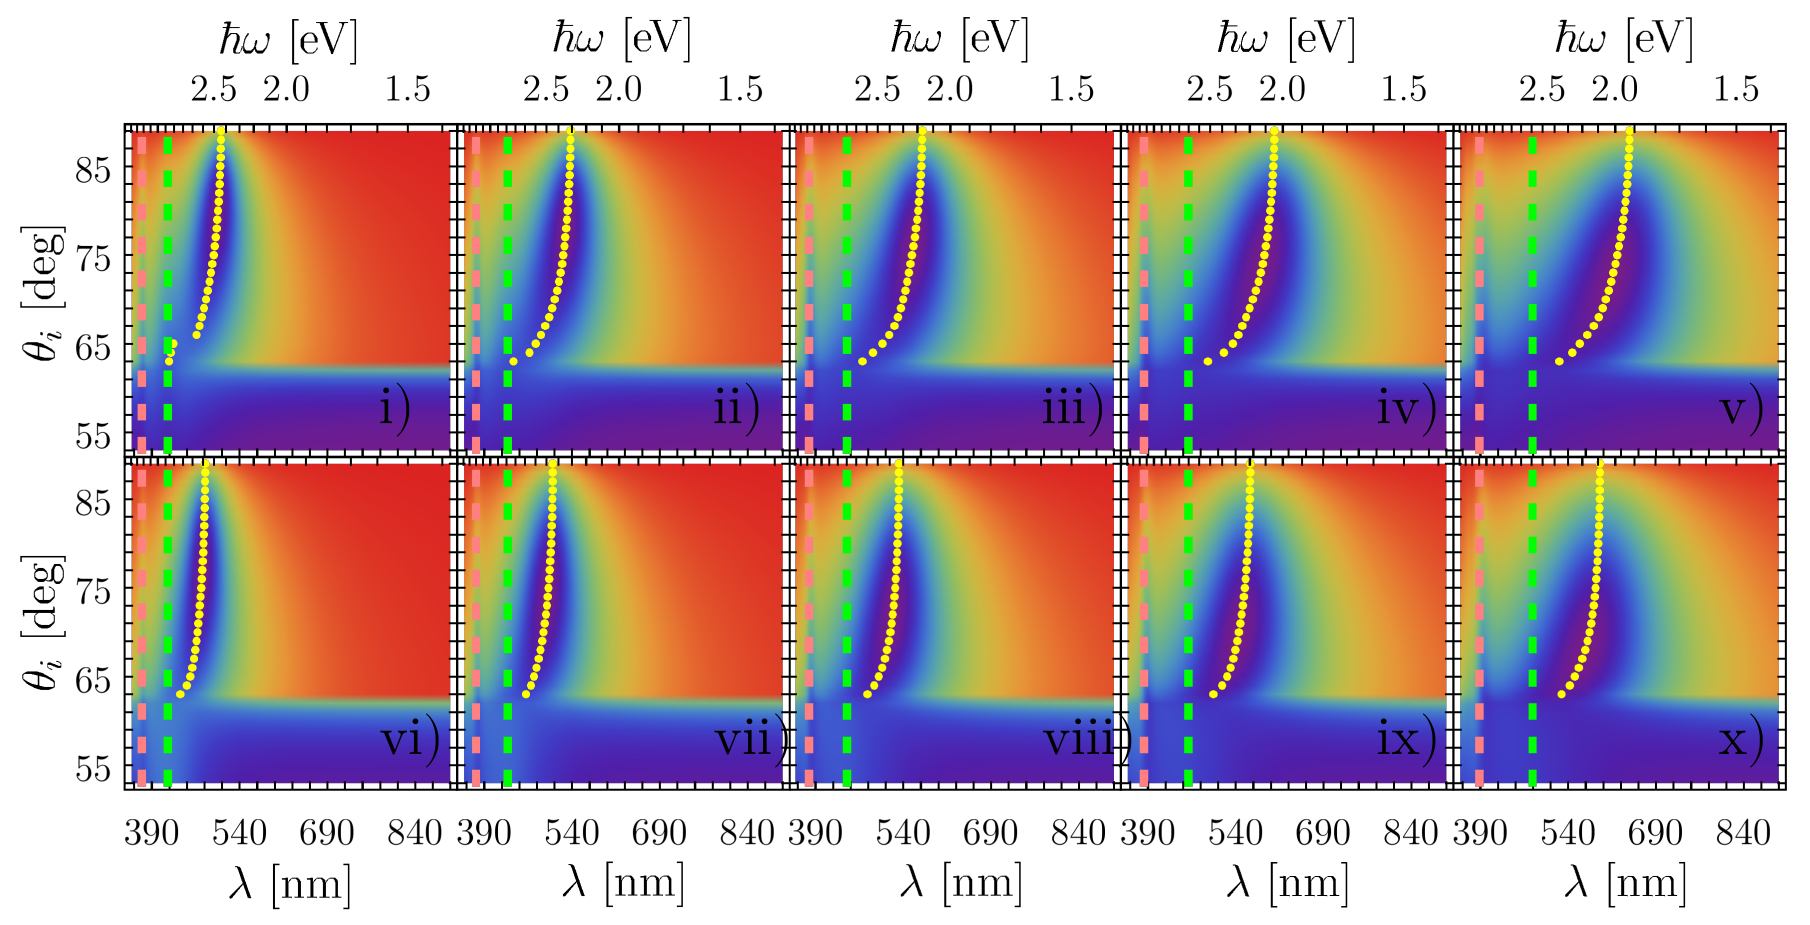
\includegraphics[scale=1]{2-Resultados/figs/9-AgrVar/0-2D_Grid}};
\node[right, inner sep=0pt] (legend) at (7.1,.15) {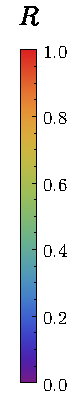
\includegraphics[scale=1, trim={00 -15 00 00}, clip]{2-Resultados/figs/0-RBar_v}};

\def\y{4.2}
	\node at(-5.2,\y){\normalsize $a = 30 $ nm};
	\node at(-2.4,\y){\normalsize $a = 35 $ nm};
	\node at(0.4,\y) {\normalsize $a = 40 $nm};
	\node at(3.2,\y) {\normalsize $a = 45 $ nm};
	\node at(6.0,\y) {\normalsize $a = 50 $ nm};

\def\xR{7}
\def\yR{2.5}	
	\node at(\xR,\yR){$R_p $};
	\node at(\xR,\yR-2.8){$R_s$};
\end{tikzpicture}\vspace*{-.5em}
	\caption{Gráficas de reflectancia de una monocapa de NPs de plata en configuración ATR como función del ángulo de incidencia $\theta_i$ y de la longitud de onda $\lambda$ (escala inferior), así como de la energía  $\hbar\omega$ (escala superior).  Las gráficas   en el renglón superior [$\mathbf{i)-v)}$] muestran los resultados para  polarización \emph{p} y las del renglón inferior  [$\mathbf{vi)-x)}$]  para polarización  \emph{s}, donde se consideró una fracción de cubierta $\Theta = 0.1$ y  NPs de radio  $a$: $30$ nm, $35$ nm, $40$ nm, $45$ nm y $50$ nm.  Las líneas verticales punteadas verdes y rosas corresponden a las SP-SPRs dipolar y  cuadrupolar, respectivamente.  Los puntos amarillos corresponden a los mínimos en $R$ para ángulos mayores a $\theta_c\approx 62.5^\circ$ y longitudes de onda mayores a la SP-SPRs dipolar.
}	\label{fig:Ag-R-Rad}	
	\end{figure}	

Los cálculos de la reflectancia de la monocapa de NPs de oro a $\theta_i=65^\circ$ y considerando ambas polarizaciones (paneles izquierdos de la Fig. \ref{fig:AuAg-Cuts-Rad-65}) muestran que el ancho de la excitación del supuesto modo colectivo disminuye  al disminuir el radio de las NPs. Por ejemplo, al comparar el resultado para $a=15$ nm (línea negra) y $25$ nm (línea amarilla) a $\lambda\approx 530$ nm. Asimismo, la presencia del supuesto modo colectivo es menos evidente para los radios mayores, como se observa para $a=35$ nm (línea turquesa), en donde el supuesto modo colectivo  se localiza en $\lambda^{exc}\approx 550$ nm para ambas polarizaciones; sin embargo, para ambas polarizaciones, cuando $\lambda<\lambda^{exc}$ la reflectancia $R$ es menor a $0.1$ por lo que el supuesto modo colectivo no es tan apreciable como para el caso de $a=20$ nm (línea naranja) en donde $R\approx 0$ en $\lambda^{exc}\approx 530$ nm y en donde  $R\approx 0.2$ para $\lambda<\lambda^{exc}$. Es decir, para ángulos cercanos al ángulo crítico, las NPs de oro de menor tamaño son más aptas para el biosensado, así como valores de $\Theta$ cercanos a $0.125$.

	\begin{figure}[h!]\centering
	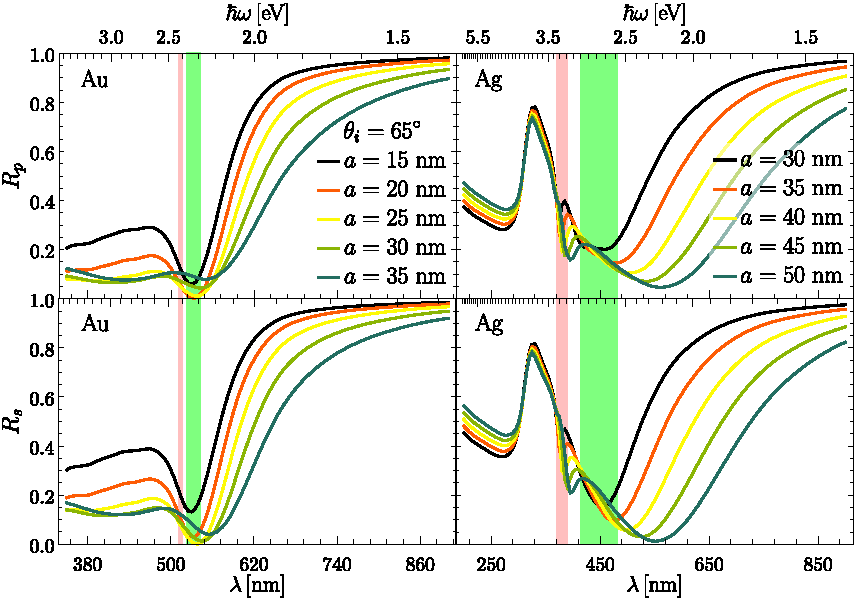
\includegraphics[scale=1]{2-Resultados/figs/8-AurVar/0-cut65_Au_Aug.pdf}\vspace*{-.5em}
	\caption{Cortes a $\theta_i = 65^\circ$ de las gráficas de reflectancia  en configuración ATR  de una monocapa de NPs esféricas de oro con $\Theta=0.125$ (Fig. \ref{fig:Au-R-Rad}) y de plata con $\Theta=0.1$ (Fig. \ref{fig:Ag-R-Rad}) como función de la longitud de onda $\lambda$ (escala inferior) y de la energía $\hbar\omega$ (escala superior). Los paneles izquierdos corresponden a los cálculos para la monocapa de NPs de oro y los derechos a los de NPs de plata; los panles superiores corresponden a la reflectancia en polarización \emph{p} y los inferiores a polarización \emph{s}. Los valores de radios $a$ considerados para la monocapa de NPs de oro fueron  $a=15$ nm, $20$ nm, $25$ nm, $30$ nm y $35$ nm, localizando las SP-SPR dipolares (región sombreada verde) entre $525\mbox{ nm}<\lambda<541\mbox{ nm}$ y las cuadrupolares  (región sombreada verde) entre $513$ nm y $514$ nm; para la monocapa de NPs de plata se escogieron los radios  $a=30$ nm, $35$ nm, $40$ nm, $45$ nm y $50$ nm, por lo que las SP-SPR dipolares se encuentran entre $417\mbox{ nm}<\lambda<479\mbox{ nm}$ y las cuadrupolares $373\mbox{ nm}<\lambda<388\mbox{ nm}$.}\label{fig:AuAg-Cuts-Rad-65}
	\end{figure}

Al observar la reflectancia de la monocapa de NPs de plata a $65^\circ$ (paneles derechos en la Fig. \ref{fig:AuAg-Cuts-Rad-65}), el efecto del ensanchamiento del supuesto modo colectivo, así como el corrimiento al rojo es más evidente comparado al caso de NPs de oro (paneles izquierdos). Esto se debe a  que los valores considerados para los radios de las NPs fueron mayores que para el oro. Para polarización \emph{s} (panel inferior derecho), el ancho del supuesto modo colectivo para un radio de $a=30$ nm (línea negra) se localiza en $\lambda^{exc}\approx 450$ nm y tiene un FWHM $\Gamma$ de $80$ nm, mientras que para un radio de $50$ nm (línea turquesa), el supuesto modo colectivo se excita a $\lambda^{exc}\approx 550$ nm y $\Gamma\approx 120$ nm, es decir, $1.5$ veces mayor en comparación al caso con $a=30$ nm. Para polarización \emph{p}, considerando NPs de plata, la detección del supuesto modo colectivo se complica en comparación al caso de polarización \emph{s} dado que los valores del $\Gamma$ son, para todos los valores de $a$ considerados, al menos $40$ nm menores para \emph{s} que para \emph{p}. No sólo hay un aumento en el ancho del supuesto modo colectivo que depende de la polarización, sino también en la forma de la resonancia: para polarización \emph{p}, los picos de resonancia, a pesar de estar localizados a los mismos valores de $\lambda^{exc}$ para el mismo valor de $a$ en polarización \emph{s},  muestran un comportamiento cualitativo distinto para $\lambda\lessapprox\lambda^{exc}$ que $\lambda\gtrapprox\lambda^{exc}$, a diferencia de los resultados para \emph{s}, donde el supuesto modo colectivo presenta un comportamiento más simétrico alrededor de $\lambda^{exc}$. A pesar de la distinta forma de la resonancia según la polarización, las resonancias a ambas polarizaciones pueden identificarse ya que la SP-SPR cuadrupolar no se traslapa con el supuesto modo colectivo y se aprecia como un mínimo en la reflectancia. Las NPs de plata de mayor tamaño y fracciones de cubierta bajas ($\Theta= 0.1$) permiten el empleo de la monocapa para el sensado al elegir ángulos cercanos a $\theta_c$, pues el supuesto modo colectivo se sintoniza en el espectro visible, además de alcanzar valores de $R$ cercanos a cero y tener formas más definidas, en comparación a valores mayores de $\Theta$ (ver Fig. \ref{fig:AuAg-Cuts-75}), sobre todo en polarización \emph{s}.

Cuando se varió el parámetro $\Theta$ manteniendo el radio de las NPsde oro y de plata fijo (Figs. \ref{fig:AuAg-Cuts-65} y \ref{fig:AuAg-Cuts-75}) se observó que para $\theta_i=75^\circ$  el supuesto modo colectivo tenía una mejor definición en comparación a $\theta_i =65^\circ$, además de sintonizarse más hacia al rojo y, para los valores de $\Theta$ seleccionados, la reflectancia disminuía. Estas características también se observan en la variación del radio de las NPs en la monocapa (Fig. \ref{fig:AuAg-Cuts-Rad-75})  con un valor de $\Theta=0.125$ para las NPs de oro (paneles izquierdos) y de $\Theta=0.1$ para las de plata (paneles derechos). Al considerar NPs de oro, la reflectancia a longitudes menores a la SP-SPR cuadrupolar (región sombreada rosa) toma valores alrededor de $0.5$  lo que contrasta con los valores a las longitudes de onda del supuesto modo colectivo $\lambda^{exc}$ en donde, para polarización \emph{p}, $R_p(\lambda^{exc})<0.025$ para radios de $a\geq 20$ nm (líneas naranja, amarilla, verde y turquesa) y, para \emph{s} $R_s(\lambda^{exc})<0.025$ cuando $a\geq 25$ nm (líneas amarilla, verde y turquesa). Adicionalmente, para los radios  $a\geq 25$ nm, que cumplen para ambas polarizaciones que $R(\lambda^{exc})<0.025$, el supuesto modo colectivo se sintoniza en el intervalo entre $\lambda\approx 520$ nm y $\lambda\approx 620$ nm, y el ancho de la resonancia es de $\Gamma \approx 100$ nm para $a=25$ nm y de $\Gamma\approx 130$ nm para $a=35$ nm. Al tener una respuesta EM semejante para radios entre $25$ nm y $35$ nm, el supuesto modo colectivo presente en una monocapa de NPs de oro, a ambas polarizaciones y considerando $\theta_i=75^\circ$, puede emplearse en para sensado ya que errores experimentales en la fabricación de las NPs no modificarían en una forma significativa la respuesta promedio.


	\begin{figure}[h!]\centering
	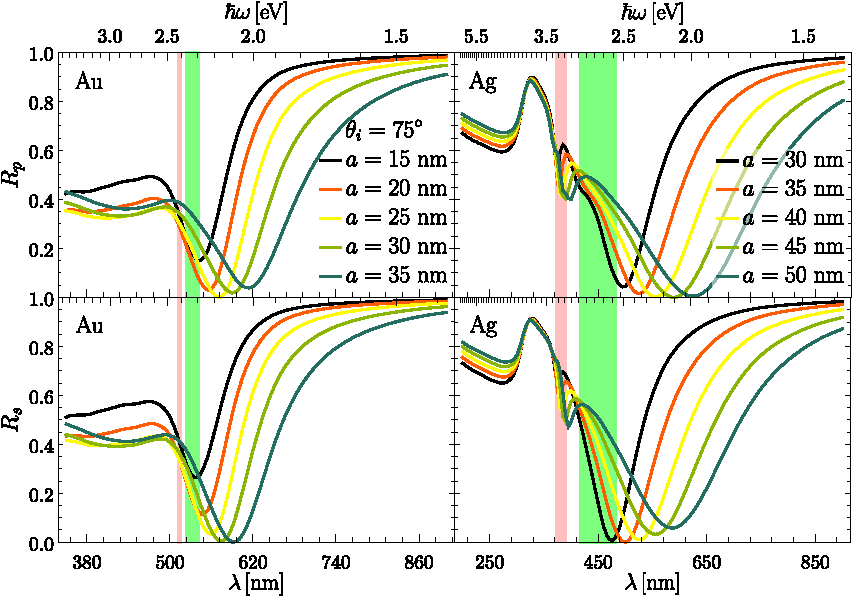
\includegraphics[scale=1]{2-Resultados/figs/8-AurVar/0-cut75_Au_Aug.pdf}\vspace*{-.5em}
	\caption{Cortes a $\theta_i = 75^\circ$ de las gráficas de reflectancia  en configuración ATR  de una monocapa de NPs esféricas de oro con $\Theta=0.125$ (Fig. \ref{fig:Au-R-Rad}) y de plata con $\Theta=0.1$ (Fig. \ref{fig:Ag-R-Rad}) como función de la longitud de onda $\lambda$ (escala inferior) y de la energía $\hbar\omega$ (escala superior). Los paneles izquierdos corresponden a los cálculos para la monocapa de NPs de oro y los derechos a los de NPs de plata; los panles superiores corresponden a la reflectancia en polarización \emph{p} y los inferiores a polarización \emph{s}. Los valores de radios $a$ considerados para la monocapa de NPs de oro fueron  $a=15$ nm, $20$ nm, $25$ nm, $30$ nm y $35$ nm, localizando las SP-SPR dipolares (región sombreada verde) entre $525\mbox{ nm}<\lambda<541\mbox{ nm}$ y las cuadrupolares  (región sombreada verde) entre $513$ nm y $514$ nm; para la monocapa de NPs de plata se escogieron los radios  $a=30$ nm, $35$ nm, $40$ nm, $45$ nm y $50$ nm, por lo que las SP-SPR dipolares se encuentran entre $417\mbox{ nm}<\lambda<479\mbox{ nm}$ y las cuadrupolares $373\mbox{ nm}<\lambda<388\mbox{ nm}$.}\label{fig:AuAg-Cuts-Rad-75}
	\end{figure}	

Para la monocapa de NPs de plata (paneles derechos de la Fig. \ref{fig:AuAg-Cuts-Rad-75}), el comportamiento es análogo al observado para la monocapa de NPs de oro. La refelctancia evaluada en las longitudes de onda del supuesto modo colectivo $\lambda^{exc}$ para la monocapa de las NPs de plata a ambas es cercana a cero mientras que a longitudes de onda menores a la SP-SPR cuadrupolar, la cual puede observase como mínimos en $R$ alrededor de la región sombreada rosa, es mayor a $0.6$, por lo que se facilitaría experimentalmente la identificación del supuesto modo colectivo. Por ejemplo, para polarización \emph{p} (panel superior derecho) para $a=40$ nm, $45$ nm y $50$ nm, el supuesto modo colectivo se localiza a $500$ nm, $530$ y $540$ nm, respectivamente, y para estos tres casos $R_p\approx 0$. Asimismo, para polarización \emph{s} (panel inferior derecho) para $a=30$ nm, $35$ nm y $40$ nm, el supuesto modo colectivo se excita a $\lambda^{exc}=460$ nm, $470$ nm y $480$ nm, respectivamente e, igualmente, $R_s\approx 0$. En general, para todos los casos de radios de NPs de plata mostrados en la Fig. \ref{fig:AuAg-Cuts-Rad-75}, la reflectancia a las longitudes de ondas del supuesto modo colectivo es menor a $0.02$ a ambas polarizaciones. Los valores de la FWHM $\Gamma$ del supuesto modo colectivo presente en la monocapa de NPs de plata y para los casos donde $R_s\approx R_p \approx 0$, son, para polarización \emph{p} de $\Gamma=80$ nm para $a=40$ nm (línea amarilla en el panel superior derecho) y $\Gamma=140$ nm para $a=50$ nm (línea turquesa en el panel superior derecho), mientras que para polarización \emph{s}, $\Gamma$ está en un rango entre $60$ nm, para $a=30$ nm (línea negra en el panel inferior derecho), y $80$ nm, para $a=40$ nm (línea amarilla en el panel inferior derecho). Al igual que con la monocapa de NPs de oro, empleando NPs de plata, el supuesto modo colectivo puede emplearse en el sensado al considerar $\Theta=0.1$ y radios de NPs entre $35$ nm y $40$ nm, pues a $\theta_i=75^\circ$, la reflectancia (para ambas polarizaciones) a las longitudes de onda  $\lambda^{exc}$ que excitan al supuesto modo colectivo es cercana a cero y representa un mínimo en la reflectancia global.

Con base en los resultados mostrados en las Figs. \ref{fig:AuAg-Cuts-75} y \ref{fig:AuAg-Cuts-Rad-75}, se propone que, para emplear una monocapa desordenada de NPs esféricas como sensor basado en el supuesto modo colectivo, se eligen los parámetros $\Theta=0.125$ y radio $a=30$ nm con NPs de oro, y $\Theta=0.1$ y $a=40$ nm con NPs de plata. Estos parámetros garantizan la validez del CSM. Finalmente, para determinar si el supuesto modo colectivo en materiales reales tiene propiedades de un modo guiado, como las LSPR reportadas en \cite{kabashin2009plasmonic} o como se observó con el CSM al considerar una monocapa de NPs cuyo índice de refracción era descrito por el modelo de Drude-Sommerfeld, se  muestran en la Fig. \ref{fig:RT-AuAg}  los cálculos de la reflectancia $R$, la transmitancia $T$ y la suma de éstas ($R+T$) de una monocapa de NPs inmersa en un medio con índice de refracción $n_m=1.33$ y soportada por un sustrato con índice de refracción $n_s=1.5$, en función del ángulo de incidencia $\theta_i$, así como de la longitud de onda $\lambda$ (escala inferior) y de la energía  $\hbar\omega$ (escala superior) de la onda plana incidente, tanto para polarización \emph{p}  [\textbf{i)}--\textbf{iii)}] como para \emph{s} [\textbf{iv)}--\textbf{vi)}]. La Fig. \ref{sfig:RT-Au} corresponde a los cálculos al considerar una monocapa de NPs de oro de radio de $30$ nm y con $\Theta=0.125$, y la  Fig. \ref{sfig:RT-Ag} a los de una monocapa de NPs de plata con radios de $40$ nm y $\Theta=0.1$, es decir, los óptimos para emplear el supuesto modo colectivo en el sensado considerando $\theta_i<80^\circ$.

\begin{figure}[h!]\centering\noindent\hspace*{-5em}
	\begin{subfigure}{.01\linewidth}\caption{}\label{sfig:RT-Au}\vspace{5.5cm}\end{subfigure}
	\begin{subfigure}{.7\linewidth}\hspace*{-.5em}
	\begin{tikzpicture}[scale=1]
\node[inner sep=0pt] (graf) at (0.05,0){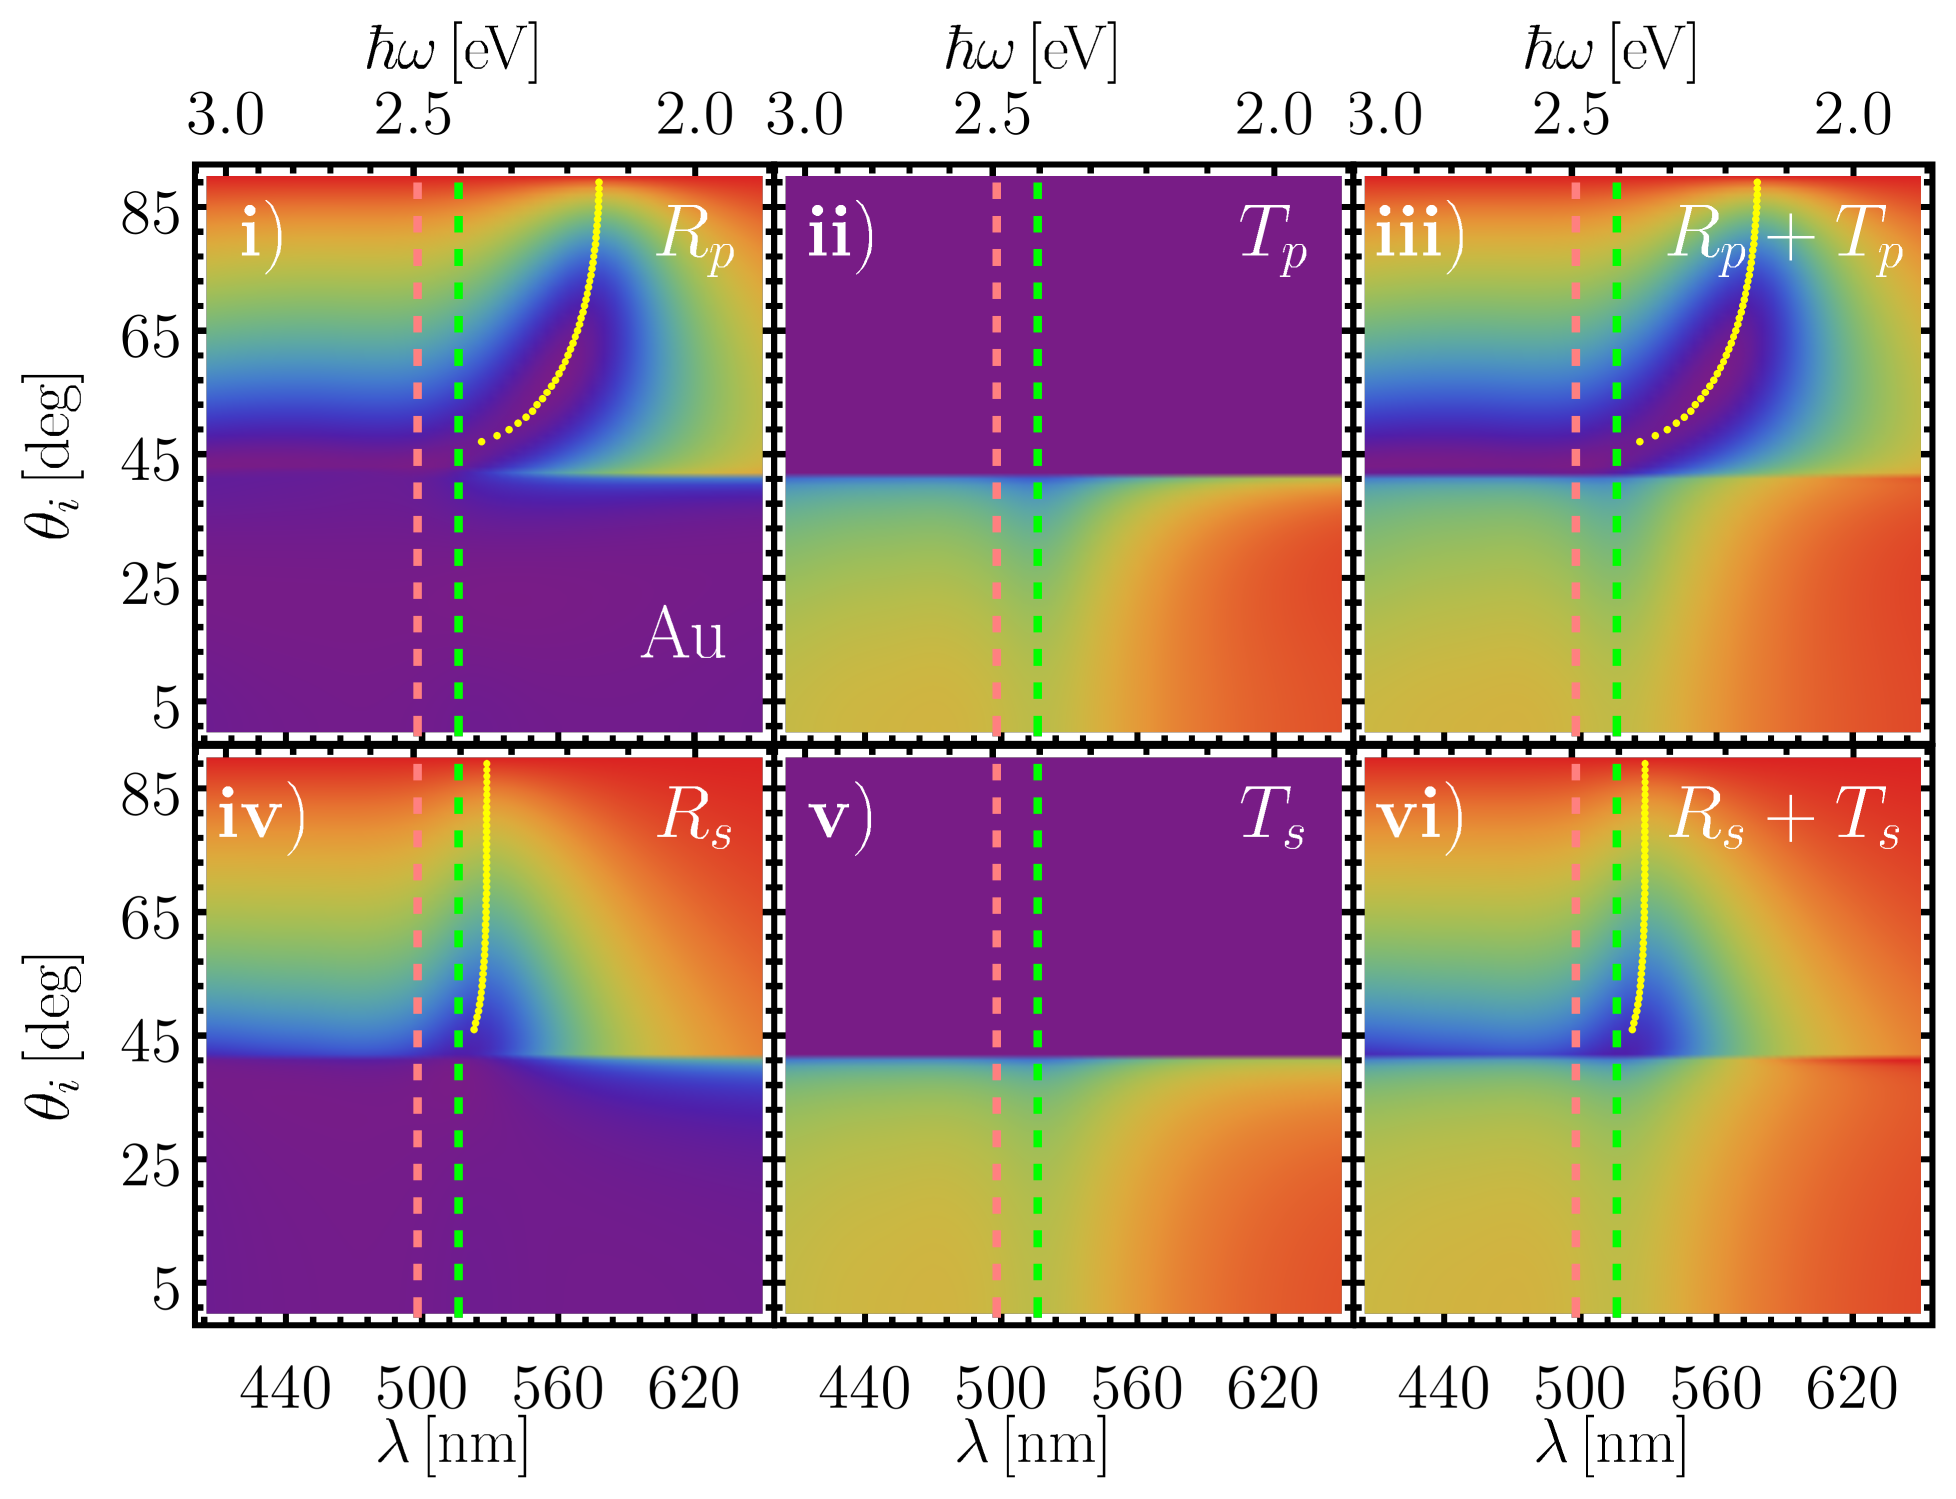
\includegraphics[scale=1]{2-Resultados/figs/10-RT-AuAg/0-2D_Grid_1.png}};
\node[right, inner sep=0pt] (legend) at (4.45,.15) {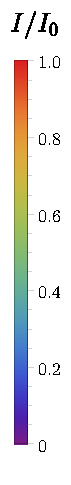
\includegraphics[scale=1, trim={00 -15 00 00}, clip]{2-Resultados/figs/0-IBar_v}};

\def\x{7.5}
	\node at(\x,1){\small $\hbar\omega_p=4.3$ eV};
	\node at(\x,0) {\small $\Theta = 0.2$};
	\node at(\x,-1) {\small $a=25$ nm};

\def\xR{4.2}
\def\yR{2.5}	
	\node at(\xR,\yR){$R_p $};
	\node at(\xR,\yR-2.8){$R_s$};
\end{tikzpicture}	
	\end{subfigure}\\ \noindent \hspace*{-4em}
	\begin{subfigure}{.01\linewidth}\caption{}\label{sfig:RT-Ag}\vspace{5.5cm}\end{subfigure}\hspace*{-.5em}
	\begin{subfigure}{.7\linewidth}\hspace*{-.5em}
	\begin{tikzpicture}[scale=1]
\node[inner sep=0pt] (graf) at (.05,0){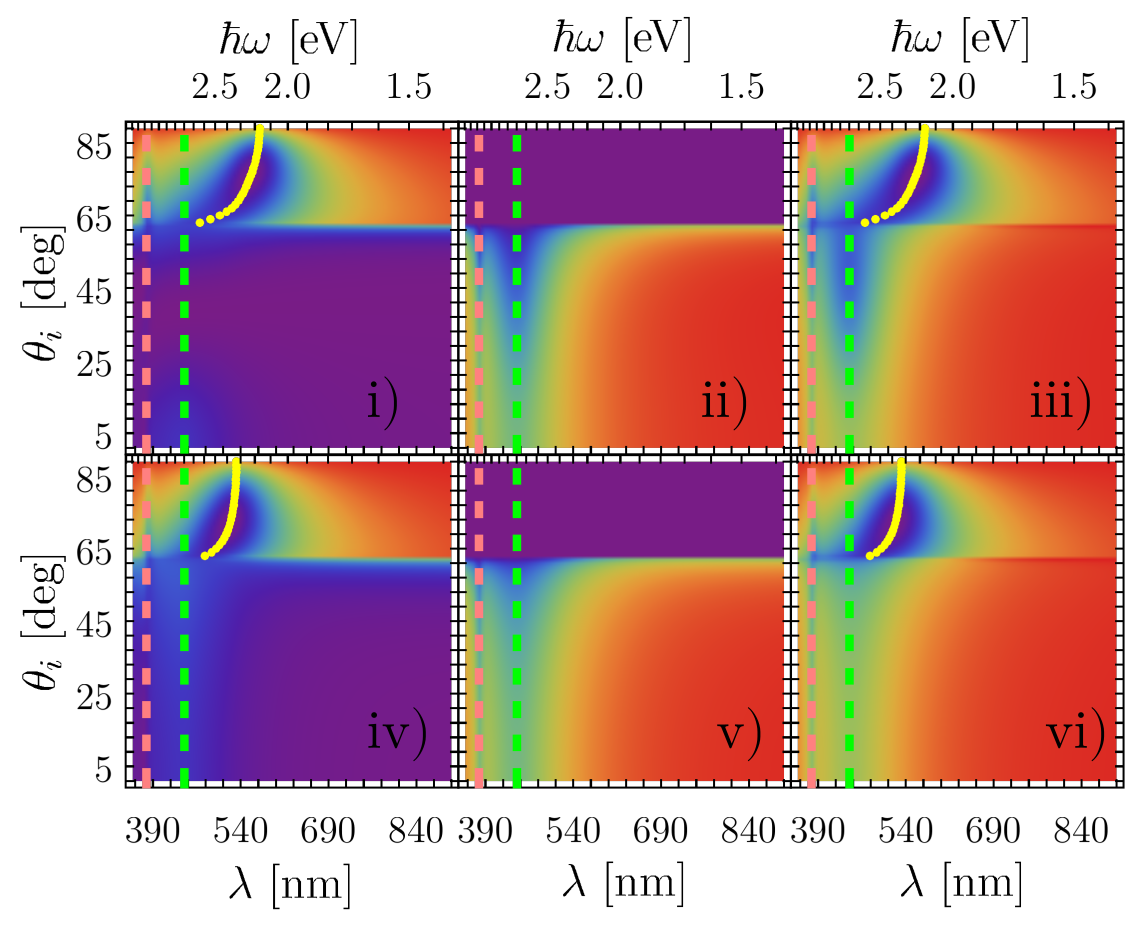
\includegraphics[scale=1]{2-Resultados/figs/10-RT-AuAg/0-2D_Grid_2.png}};
\node[right, inner sep=0pt] (legend) at (4.4,.15) {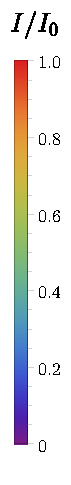
\includegraphics[scale=1, trim={00 -15 00 00}, clip]{2-Resultados/figs/0-IBar_v}};

\def\x{7.5}
	\node at(\x,1){\small $\hbar\omega_p=10$ eV};
	\node at(\x,0) {\small $\Theta = 0.3$};
	\node at(\x,-1) {\small $a=30$ nm};

\def\xR{4.2}
\def\yR{2.5}	
	\node at(\xR,\yR){$R_p $};
	\node at(\xR,\yR-2.8){$R_s$};
\end{tikzpicture}
		\end{subfigure}\vspace*{-.5em}
	\caption{Gráficas de reflectancia $R$, transmitancia $T$ y la suma de éstas $R+T$   en configuración ATR de una monocapa de NPs esféricas como función del ángulo de incidencia $\theta_i$ y de la longitud de onda $\lambda$ (escala inferior) así como de la energía de la onda plana incidente en unidades de $\hbar\omega$ (escala superior), considerando \textbf{a)} NPs de oro de radio $a=30$ nm y fracción de cubierta $\Theta$ de $0.125$, y \textbf{b)} NPs de plata de radio $a=40$ nm y $\Theta=0.1$.  Las gráficas   en el renglón superior [$\mathbf{i)-ii)}$]  muestran los resultados de reflectancia para  polarización \emph{p} y las del renglón inferior  [$\mathbf{iv)-vi)}$] para polarización  \emph{s}. Las líneas verticales punteadas verdes corresponden a la SP-SPRs dipolar ($\lambda\approx 531$ nm y $\lambda\approx 444$ nm para las NPs empleadas de oro y plata, respectivamente), y las rosas a la SP-SPR cuadrupolar ($\lambda\approx 514$ nm y $\lambda\approx 383$ nm para las NPs de oro y de plata, respectivamente). Los puntos amarillos corresponden a los mínimos en $R$, y $R+T$ para ángulos mayores a $\theta_c\approx 62.5^\circ$ y longitudes de onda mayores a la SP-SPRs dipolar. }\label{fig:RT-AuAg}
	\end{figure}	

Los resultados de $R+T$, tanto para la monocapa de NPs de oro (paneles \textbf{iii)}\textbf{vi)} en la Fig. \ref{sfig:RT-Au}) como para las de plata (paneles \textbf{iii)}\textbf{vi)} en la Fig. \ref{sfig:RT-Ag}), muestran un comportamiento análogo al observado en el caso donde se emplearon las funciones dieléctricas tipo Drude para las NPs de la monocapa: la reflectancia a las longitudes de onda del supuesto modo colectivo (puntos amarillos) es cercana a cero, además de que la transmitancia a esas mismas longitudes de onda es cero. Es decir, la luz a las longitudes de onda de excitación del supuesto modo guiado no se refleja y tampoco se transmite. Dado que la extinción de luz de una partícula esférica de oro de $a=30$ nm inmersa en un medio con índice de refracción igual a $1.33$, ocurre a $\lambda= 514$ nm, y no a las longitudes de onda del supuesto modo colectivo, el decremento en la reflectancia no puede deberse a la absorción. Análogamente, una NP de plata de $a=40$ nm presenta su máximo de extinción a $383$ nm, por lo que no puede haber absorción a las longitudes de onda del supuesto modo colectivo. Por tanto, el supuesto modo colectivo presenta las propiedades de un modo guiado cuando se consideran materiales realistas para las NPs.

El supuesto modo colectivo, observado en una monocapa de NPs con una función dieléctrica tipo Drude, también aparece al considerar las funciones dieléctricas experimentales para el oro y la plata de \cite{johnson1972constants}, con sus respectivas correcciones por tamaño. Al considerar una monocapa de NPs de oro de radio $a=30$ nm con una fracción de cubierta $\Theta=0.125$ y una de NPs de plata de $a=40$ nm y $\Theta=0.1$ (ver Fig. \ref{fig:RT-AuAg}), es posible emplear el supuesto modo colectivo para el sensado, considerando un intervalo para el ángulo de incidencia $70^\circ<\theta_i<80^\circ$ (ver Fig. \ref{fig:AuAg-Cuts-Rad-75}). Para evaluar el uso del supuesto modo colectivo en el sensado, en la siguiente sección se estudia  respuesta del supuesto modo colectivo ante cambios del índice de refracción de la matriz $n_m$ y, a su vez, se compara la respuesta del supuesto modo colectivo con la de biosensores plasmónicos comerciales, los cuales emplean la excitación del plasmón polaritón de superficie en una una película de $50$ nm (de oro o de plata de $50$ nm) \cite{estevez2014trends,svedenhal2009refractrometric}, así como con prepuestas de sensores nanoestructurados basados en las resonancias de superficie localizadas \cite{svedendahl2009refractometric} y en las LSPRs \cite{danilov2018ultra}.
